\section{Related Work}
\subsection{Diffusion models for Video Generation}
Diffusion models have demonstrated an impressive capability to generate high-quality video samples. Previous research~\cite{ho2022video, ho2022imagen, singer2022make,khachatryan2023text2video,zhang2023controlvideo} commonly use video diffusion models~(VDMs) that incorporate temporal convolutional and attention layers into the pre-trained image diffusion models. Subsequently, VideoCrafter~\cite{Chen2023VideoCrafter1OD} and SVD~\cite{DBLP:journals/corr/abs-2311-15127} expand the application of video diffusion models to larger datasets, while TF-T2V~\cite{wang2024tf} directly learns from extensive text-free videos. Nonetheless, these methods encounter limitations in generating long videos, owing to the inherent constraints on capacity and scalability within the UNet design. Conversely, DiT-based models~\cite{sora2024, OpenSora,DBLP:journals/corr/abs-2405-04233, yang2024cogvideox, polyak2024movie} can directly generate videos extending up to tens of seconds. Sora~\cite{sora2024} converts visual data into a unified representation, facilitating large-scale training and enabling the generation of 1-minute high-definition video. Vidu~\cite{DBLP:journals/corr/abs-2405-04233} is capable of generating both realistic and imaginative videos in various aspect ratios. CogVideoX~\cite{yang2024cogvideox}  introduces an expert diffusion transformer model that generates videos from text prompts or images, along with an effective text-video data processing pipeline that enhances video caption quality. 
%Movie Gen~\cite{polyak2024movie} introduces a collection of foundational models that generate high-quality videos with different aspect ratios and synchronized audio. 
%For our study, we adopt OpenSorav1.2 ~\cite{OpenSora} as the foundational model, which is an open-source alternative to Sora.


\begin{figure*}[!t]
    \centering
    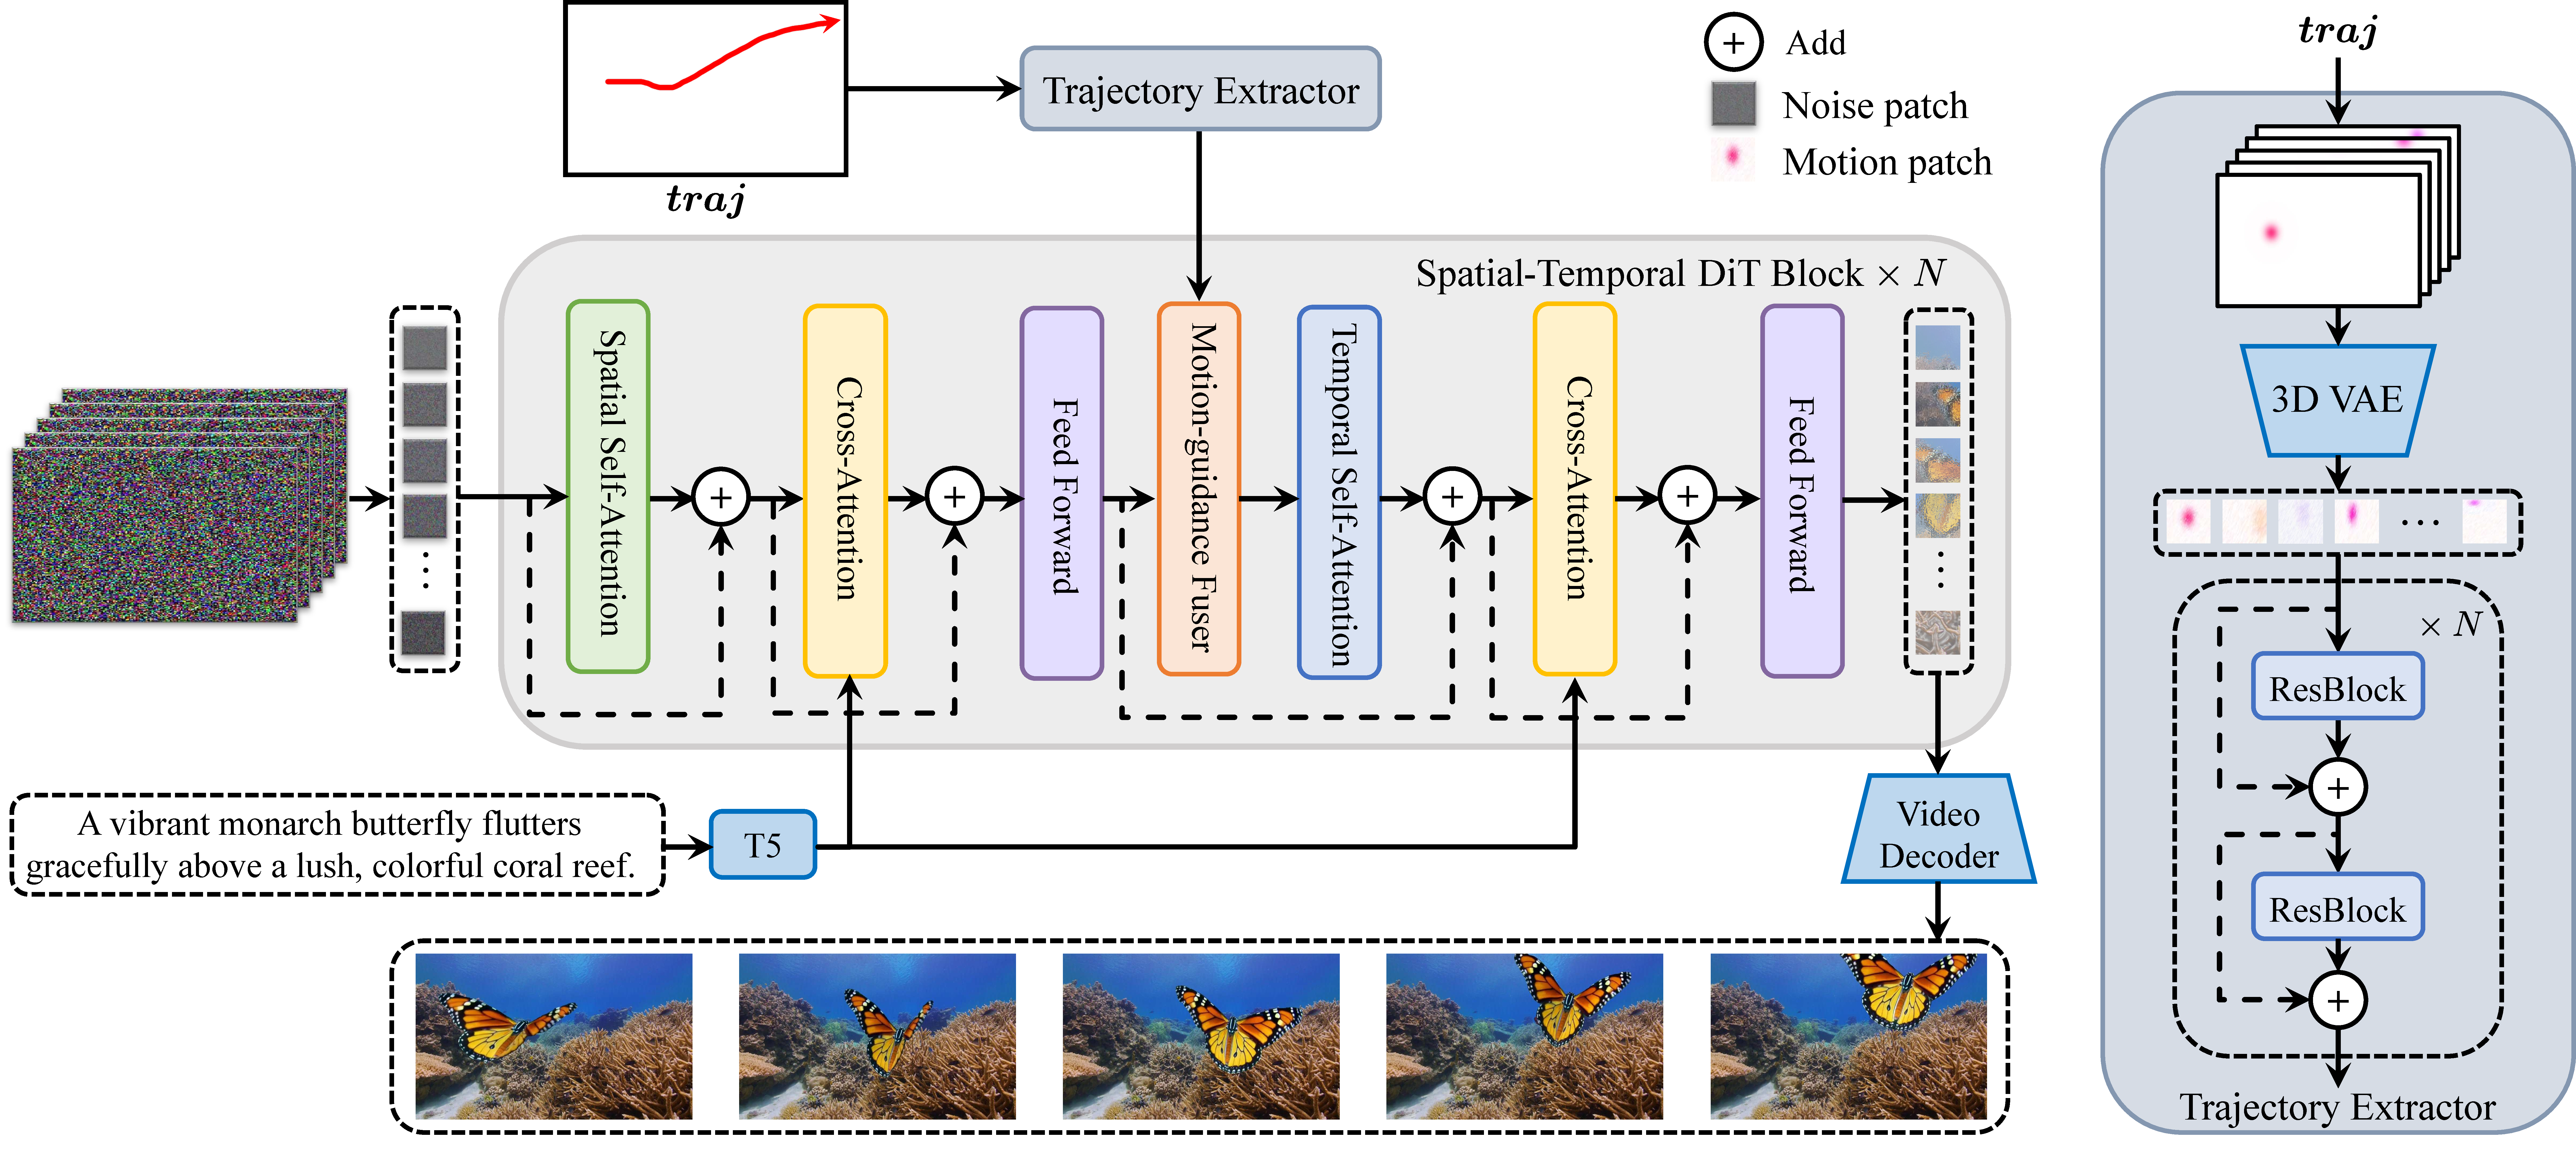
\includegraphics[width=0.95\textwidth]{images/pipeline.pdf}
    \caption{
    Overview of the Tora Architecture. We introduce two novel modules: the Trajectory Extractor and the Motion-guidance Fuser. The Trajectory Extractor uses a 3D motion VAE to embed trajectory vectors into the same latent space as video patches, preserving motion information across frames. It then employs stacked convolutional layers to extract hierarchical motion features. The Motion-guidance Fuser utilizes adaptive normalization layers to integrate these multi-level motion conditions into the corresponding DiT blocks, ensuring that generated videos consistently follow defined trajectories. Our method leverages the scalability of DiT, enabling the creation of motion-controllable videos of extended duration.
    }
    \label{fig:3}   
\end{figure*}


\subsection{Motion control in Video Generation}
To better control motion in generated videos,  a multitude of studies have endeavored to introduce diverse motion signals in VDMs.
Pioneering works like MotionDirector~\cite{DBLP:journals/corr/abs-2310-08465} and VMC~\cite{jeong2024vmc} have utilized reference videos to extract motion patterns applicable to diverse video generations. VideoComposer~\cite{wang2023videocomposer} expands upon this by adopting depth maps, sketches, or motion vectors from references as conditional inputs for motion control. Nonetheless, these methodologies are limited to reproducing existing motion patterns. Conversely, approaches that leverage trajectories~\cite{mou2024revideoremakevideomotion,geng2024motionpromptingcontrollingvideo,shi2024motioni2vconsistentcontrollableimagetovideo,yin2023dragnuwa,wang2024motionctrl,DBLP:journals/corr/abs-2401-00896} or bounding boxes~\cite{yin2023dragnuwa,DBLP:journals/corr/abs-2311-12886, wang2024motionctrl} in video generation promise greater adaptability and user accessibility.
DragNUWA~\cite{yin2023dragnuwa} breaks new ground by integrating trajectory-based conditioning into VDMs, facilitating complex camera and object movements. AnimateAnything~\cite{DBLP:journals/corr/abs-2311-12886} employs motion masks for precise control over the moving regions. DragAnything~\cite{wu2024draganythingmotioncontrolusing} uses the object mask to generate entity representations for achieving motion control. %TrailBlazer~\cite{DBLP:journals/corr/abs-2401-00896}, employs explicit attention mechanisms to maneuver generated objects along precise trajectories. 
MotionCtrl~\cite{wang2024motionctrl} facilitates more flexible control, allowing separate adjustment of both camera movements and individual object motions.
However, all of them yield noticeable artifacts in both motion consistency and visual presentation when applied to longer sequences.  In contrast, our method first integrates trajectories into DiT architecture, which enables closer adherence to the physical world.

